\documentclass{article} % For LaTeX2e
\usepackage{nips14submit_e,times}
\usepackage{hyperref}
\usepackage{url}
\usepackage{graphicx}
\usepackage[utf8]{inputenc}
\usepackage[francais]{babel}
\usepackage{lmodern}
\usepackage[T1]{fontenc}
\usepackage{xcolor}
\usepackage{amsmath, amssymb, amsthm, mathalfa}
\usepackage{caption}
\usepackage{geometry}
\usepackage{thmbox}
\usepackage{enumerate}
\usepackage{subcaption}
\usepackage{bbm}
\bibliographystyle{plain}


\title{SSL via Locally Sensitive Hashing (LSH)}


\author{
Timothée Lacroix \\
MVA student - ENS Cachan\\
\texttt{timothee.lacroix@ens.fr} \\
\And
Judith Abécassis \\
MVA student - ENS Cachan \\
\texttt{judith.abecassis@ens.fr} \\
}

% The \author macro works with any number of authors. There are two commands
% used to separate the names and addresses of multiple authors: \And and \AND.
%
% Using \And between authors leaves it to \LaTeX{} to determine where to break
% the lines. Using \AND forces a linebreak at that point. So, if \LaTeX{}
% puts 3 of 4 authors names on the first line, and the last on the second
% line, try using \AND instead of \And before the third author name.

\newcommand{\fix}{\marginpar{FIX}}
\newcommand{\new}{\marginpar{NEW}}

%\nipsfinalcopy % Uncomment for camera-ready version

\begin{document}


\maketitle

\begin{abstract}
Several Semi-Supervised Learning algorithms make use of unlabeled examples to estimate a manifold through a discrete graph that represents it well. Building an exact graph is at least $\mathcal{O}(n^2)$ operation, which is intractable for larger scale problems. A sensible way of dealing with this issue is to use approximate nearest neighbors search to find the edges of a k-NN (hence sparse) graph. Using Locally Sensitive Hashing will lead to some errors in the graph construction. This work is a study of how those errors will affect the generalization bound on the Harmonic Function Solution for label propagation on a graph. Practical results on the CIFAR dataset will complement those theoretical results.
\end{abstract}


\section{Semi-Supervised Learning Framework}

In this work, we are interested in semi-supervised learning (SSL) settings on a large number of points. The goal of SSL is to leverage a large number of unlabelled data points to estimate the underlying manifold geometry. We will call this manifold $\mathcal{M}$ in the rest of this work. Of our $n$ data points, we only have $n_l$ labelled points and $n_u$ unlabelled points. The goal is to propagate labels over the manifold.\\

It is reasonable to assume that for a good feature space, the labelling function will be smooth over $\mathcal{M}$. This intuition leads us to consider Harmonic Function Solutions : 
$$\ell^* = argmin_{\ell \in \mathcal{R}^n} (\ell-y)^TC(\ell-y) + \ell^TQ\ell$$
Where $(\ell-y)^TC(\ell-y)$ ensures that labelled points are still well classified, and $\ell^TQ\ell$ is responsible for the smoothness of the solution over the graph. If data points are representative of $\mathcal{M}$, and the graph is well estimated, this should lead to a smooth solution over $\mathcal{M}$ as well. The fact that the graph Laplacian is a good estimator of the diffusion process over the manifold isn't trivial and has been studied (\cite{ting2011analysis}, \cite{hein2006graph}). In our case, \cite{ting2011analysis} showed the convergence of the k-NN solution under good assumptions.

Two problems arise when the problem grows in scale :
\begin{itemize}
\item Constructing the graph itself requires $\mathcal{O}(n^2)$ distance comparisons,
\item Inverting the Laplacian matrix is around $\mathcal{O}(n^3)$.
\end{itemize}

We are interested here in a solution to the first problem, in the form of approximate nearest neighbors. The hope is that the error introduced in the graph by approximate neighborhood will be small enough. The obtained graph is then used to compute the soft harmonic function (HFS) in an iterative way.

Other attempts to address semi-supervised learning framework with a large number of nodes have been proposed. We have in particular considered the Fergus algorithm \cite{fergus2009semi} to compare to LSH. Fergus's idea is to estimate the density of points from available data. This estimated density can then be used in combination with results from the spectral graph theory to compute accurate numerical approximations to the eigenvectors and eigenfunctions of the normalized graph Laplacian and use these approximations to easily propagate labels through the whole graph.


\section{Locality Sensitive Hashing}
\subsection{Principle}

The idea behind LSH is that we want to represent complex data (a lot of points described by high-dimensional vectors) in a more simple way. To achieve that, a finite number of indexes, smaller in memory than the original high-dimensional describers, are used to represent all points. This is a simple hash table ; the additional constraint is that close points should have the same index. In that way, obtaining reasonably close points from the query only requires retrieving points labeled with the same index, and find the closest among them, instead of searching the entire database. The approximation is due to the fact that there is a probability that two close points end up in different bins.

LSH attempts to regroup points that are nearby in small buckets. Then, in each buckets, we can find the closest neighbors. Two points that are close by can fall on the other side of a bin, leading to errors. The main idea is to see that two points that are close will stay close when projected on many directions, but two points that are far apart will often stay that way when projected. We define $h^w_{a,b}$ to be the bin number for point $v$, whith a bin size of $w$, $b \sim \mathcal{U}([0,w])$ and $a \sim \mathcal{N}(0,1)$.
$$h_{a,b}^w(v) = \lfloor \frac{ a \cdot v + b}{w} \rfloor$$

This is fast to evaluate, and leads to a natural representation for a point that can be hashed easily.  An important requirement is that the hash function that maps each point to an index is fast to compute: typically, a scalar product is an efficient way to compute hash functions, and the obtained dot product can be discretized by taking the floor function. By taking a random vector, and computing the dot product of all data points with that vector, one can obtain a hash function. It can happen that remote points will end up with the same index. To reduce the probability that it happens, one can repeat the process, and draw several random vectors. The number of projections should not be to high either, as in that case, all points would have different indices, and this would make the performance of approximate nearest neighbors decrease.

\subsection{Accuracy}
As shown in \cite{slaney2008locality}, we can show that in an $L_2$ space, the probability for two point $p$ and $q$ at distance $u$ to be classified in the same bucket is 
\begin{align*}
  p^w(u) &= \int_0^w \frac{1}{u}\left( \frac{1}{\sqrt{2\pi}}\exp(-\frac{t^2}{2u^2})\right)\left(1-\frac{t}{w}\right)dt
\end{align*}
In the rest of this work, we assume there exists a function $P^w:\mathcal{R}\mapsto [0,1]$ that represents the probability that two points will end up in the same bin in the final LSH implementation.

\section{Theory}
\subsection{Strategy}
Let $L^*$ and $\hat{L}$ be the normalized laplacians for the k-NN graph and approximate k-NN graph. With the usual notation, let $Q = L+\gamma_gI_n$ and $C$ be diagonal with coefficient $c_\ell$ for labelled node and $c_u$ for unlabelled nodes.
$$\ell^* = (C^{-1}Q^* + I_n)^{-1}y \quad \hat{\ell} = (C^{-1}\hat{Q} + I_n)^{-1}y$$
This leads to 
$$ \mathbb{E}[\Arrowvert\ell^*-\hat{\ell}\Arrowvert_2] \leq \frac{\sqrt{n_\ell}}{c_u\gamma_g^2}\mathbb{E}[\Arrowvert(L^*-\hat{L})\Arrowvert_F]$$
Controlling the error $\mathbb{E}[\Arrowvert(L^*-\hat{L})\Arrowvert_F]$ gives a direct control over the generalization error of this SSL algorithm. This control only needs to be $\mathcal{O}(1)$ to get a satisfying $\mathcal{O}(n^{-1/2})$ error term.

\subsection{Controlling the frobenius norm}
Let $x, y, z \in \mathcal{M}$, $x$ is our reference node, $y$ is its true closest neighbor, and $z$ is the closest neighbor returned by LSH (further away from $x$ than $y$). See figure~\ref{degeu} for a representation. Then we can write the expected error contribution to the frobenius norm (without normalizing the Laplacian):
$$\mathbb{E}[\Arrowvert x-y\Arrowvert_2^2 + \Arrowvert x-z\Arrowvert_2^2] = \int_y \int_z (1-P^w(y))P^w(z)dydz$$
Where the density of data points over $\mathcal{M}$ is hidden in the two differentials. This density, the diameter of the manifold, and the decay of $P^w$ will be heavily involved in bounding this term. The faster the decay, the smaller $(1-P^w(y))P^w(z)$ will be.
\begin{figure}[ht!]
 \centering
 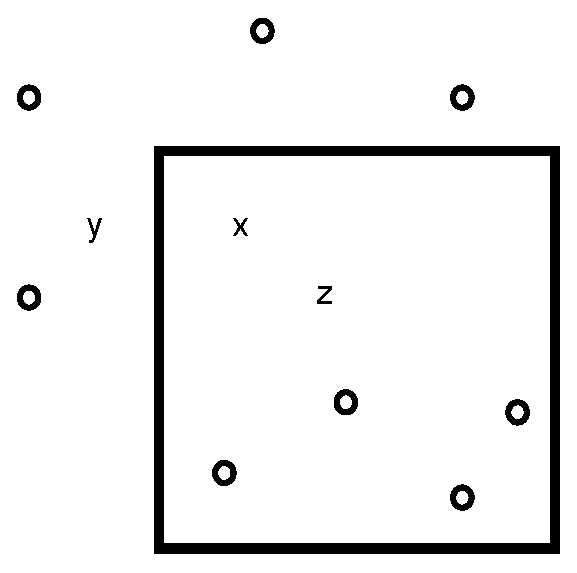
\includegraphics[width=0.45\textwidth]{figures/dessin_degeu.eps} 
 \caption{Example situation in $2D$ with grid buckets. The closest neighbor should be $y$ but it's on the other side of the bucket's boundary, hence LSH will return $y$ as the closest neighbor.}
 \label{degeu}
\end{figure}

\section{Experiments}

\subsection{Investigating the frobenius norm difference}
Since we couldn't get a theoretical bound in time, we decided to try to see how big the difference was, and how it evolved with different parameters. We expect to get a linear dependence in $k$ the number of neighbors. The error should decrease and the query time increase as the number of bucket increases (since this leads to smaller bins, hence more boundary issues, but less neighbors in each bin). This implies a need to compromise between speed and accuracy. Since the error is heavily linked with the underlying manifold, we would suggest to run a few similar tests on each specific dataset before choosing adequate parameters for the LSH. Our results for CIFAR are shown in figure~\ref{figure_test_theoriques}.

\begin{figure}[!ht]
 \begin{subfigure}{0.43\textwidth}
   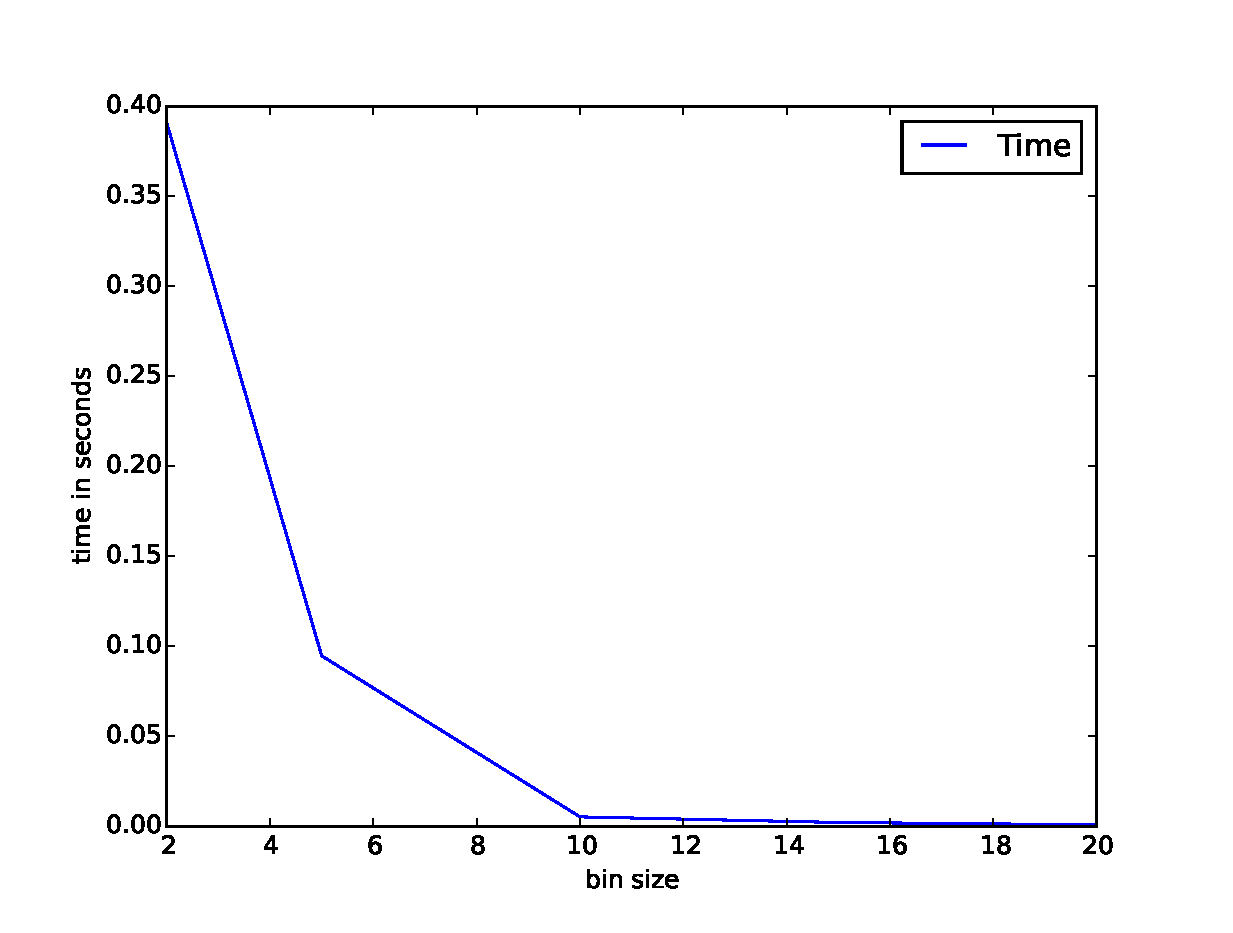
\includegraphics[width=\textwidth]{figures/time_binsize.eps}
   \caption{Average time for a nearest neighbor query, as the number of bucket increases}
 \end{subfigure}\hfill
 \begin{subfigure}{0.43\textwidth}
   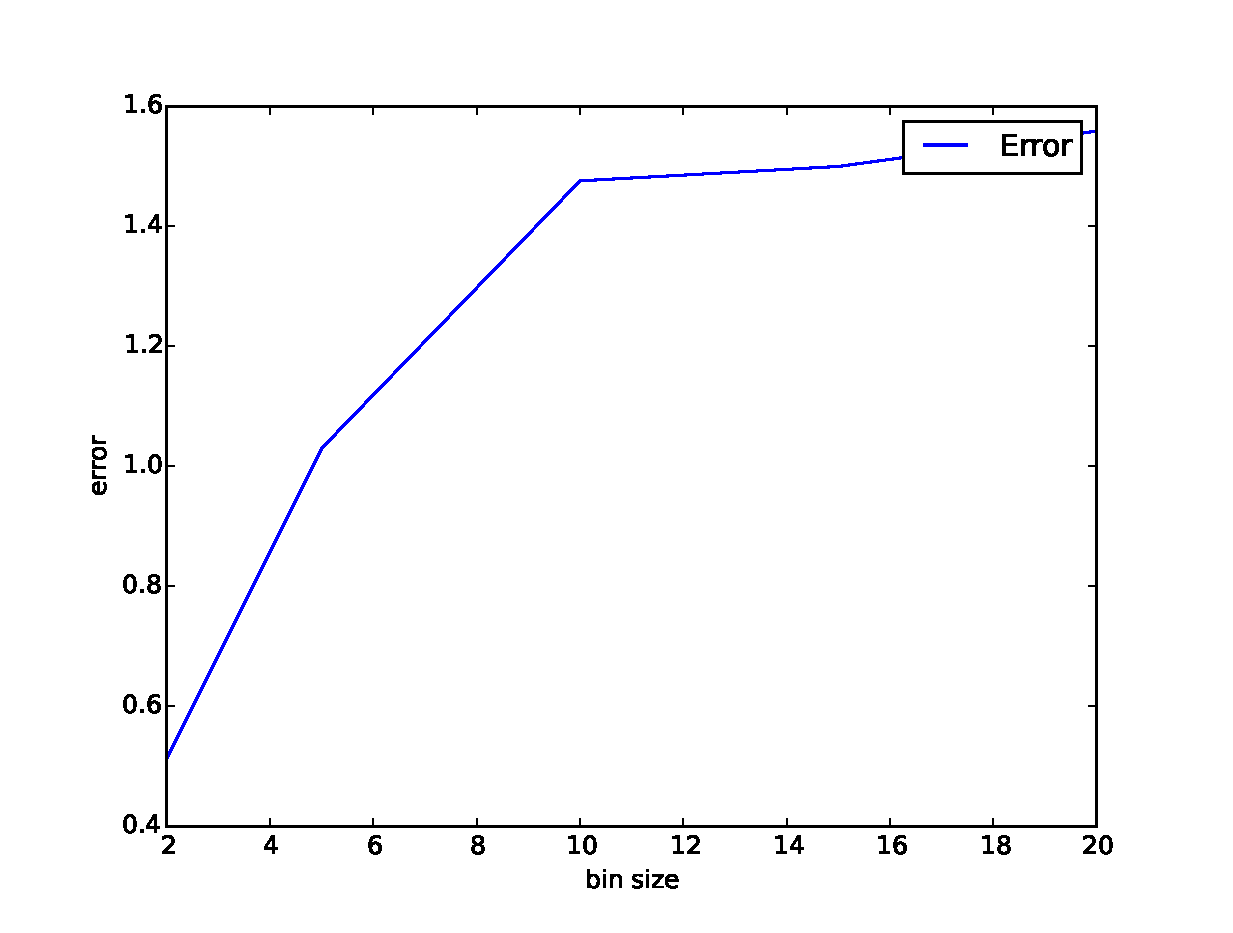
\includegraphics[width=\textwidth]{figures/error_binsize.eps}
   \caption{Average normalized error for an approximated line of the Laplacian and an exact line, as the number of bucket increases}
 \end{subfigure}\hfill
 \centering
 \begin{subfigure}{0.43\textwidth}
   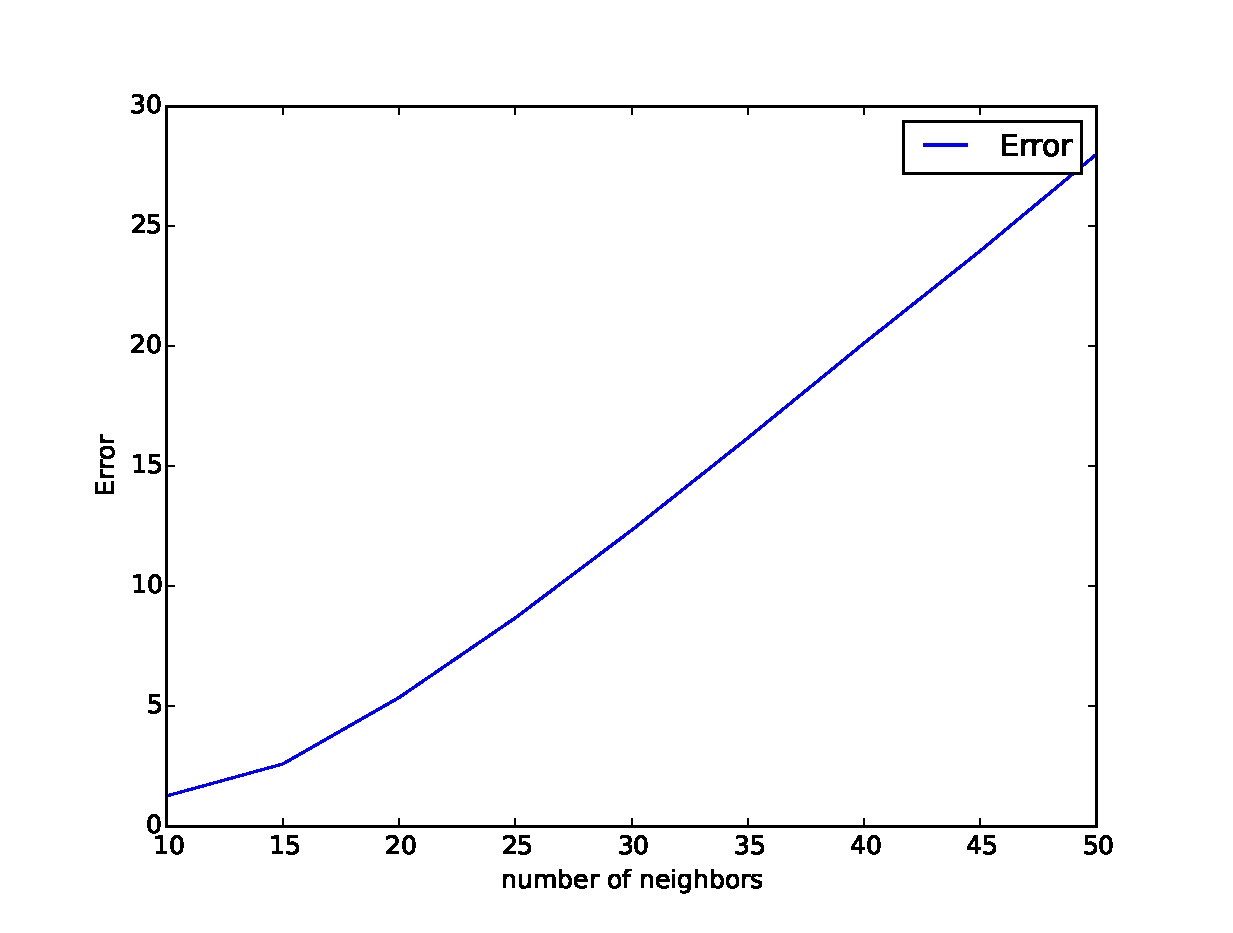
\includegraphics[width=\textwidth]{figures/error_k.eps}
   \caption{Average normalized error for an approximated line of the Laplacian and an exact line, as the number of neighbor increases}
 \end{subfigure}\hfill
 \caption{Some metrics on the error contribution of LSH on the CIFAR dataset}
 \label{figure_test_theoriques}
\end{figure}


\subsection{Presentation of the tinyImages and CIFAR100 dataset}
To allow comparison with the LSH followed by HFS to Fergus algorithm, we have used similar data to evaluate the performance, i.e., we have used the Tiny Images Dataset, which is composed by around 80 million images, enriched with Gist descriptor for each image. We first applied a PCA to reduce the dimensions of the features to 32. then we considered only a subset of the images, labelled with CIFAR labels. We restricted ourselves to the CIFAR100 dataset, which consists in 100 different classes, each one represented by 600 images (500 for training and 100 for testing).
 
\subsection{Testing setting}
To evaluate the performance of algorithms, we have used a setting similar to the one used by Fergus et al. (citer fergus). $C=16$ classes are selected. For each of these classes, $t$ positive and $2t$ negative points are labeled for each other classes. $t$ varies from 0 to 100. The rest of labels are unknown. A learning method (LSH+HFS or Fergus) is then applied to obtain the labels for the rest of the points. $300$ points are then selected to measure the performances, for each class $c$: 100 with $c$ label, and 200 with a different label. From this, for each class, the precision at $15\%$ of recall is measured, and averaged on the $C$ classes. This final number is used as a performance score for the method for this number of labeled examples.


\subsection{Fergus algorithm as a baseline}
To have a baseline comparison for the LSH+HFS method we are trying to apply, we have first attempted to reproduce results obtained with Fergus algorithm for the same testing setting (which is slightly different from ours, they have used a slightly less constrained selection of the classes, and have used 126 classes, instead of the 100 we have selected). Moreover, in the original experiment, they have kept the first 64 principal components, and us only 32 due 
to computational limitations. Results are presented in Figure \ref{variation}, along with the LSH+HFS results. We have kept the metrics and the results presentation from the original publication.

\begin{figure}[!h]
  \hspace{-3cm}
  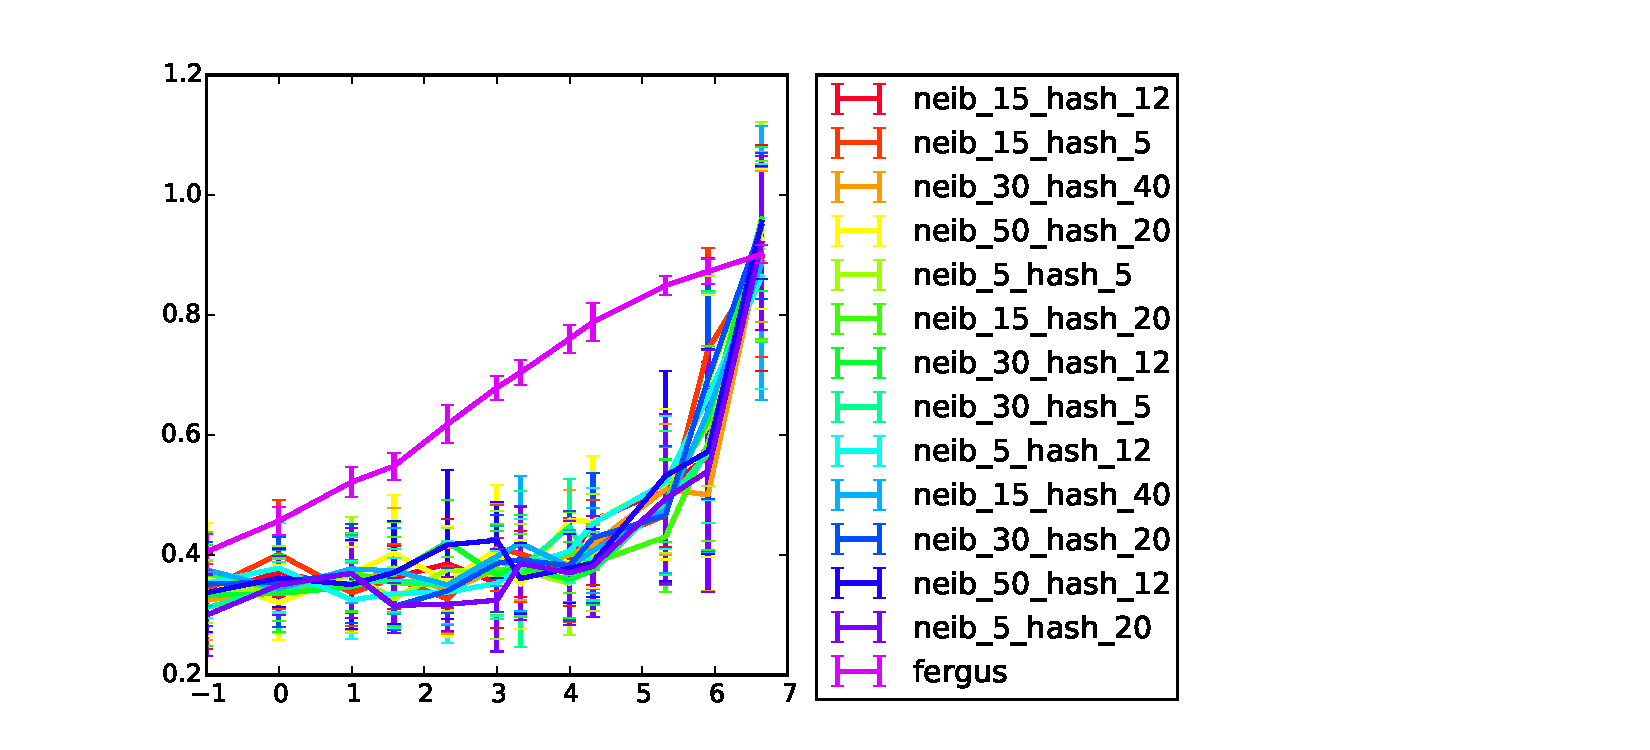
\includegraphics[width=1.8\textwidth]{method_comp.pdf}
  \caption{Performance measures for different parameters}
  \label{variation}
\end{figure}

\subsection{Results}
We have applied this setting to the method LSH+HFS. Due to computational limitations, we only used data points from 25 classes, and only $C=10$ classes were considered. We then explored a large panel of number of neighbors and number of projections for the process of building the graph from data. We obtained the following results:



We can see poor performance, barely better than random for low numbers of labeled points. Then, above 40 labeled positive points per class, performance increases significantly. We can assume that this lack of efficiency might be due to the reduction of the dataset, which certainly lowers the density of points and hence, the reliability of the ANN computation. This is also supported by the fact that values of parameters have little influence over performance. 

\subsection{Limitations of our experimental setting}
To conduct experiments concerning LSH+HFS methods, we have used the existing implementation in Python, in the \texttt{Graphlab} and \texttt{Nearpy} packages. The algorithm was very slow to run (more than 6 hours on a reduced dataset containing only 15.000 points instead of the original 60.000). We believe that \texttt{Graphlab} omptimizations were efficient for even larger data, and might be suboptimal for smaller datasets. To only run the propagation step once, we have slightly modified the problem, and instead to have 1 for positive, -1 for negative and 0 for others, we have set 1 for positive, and 0 in any other case. For example, in the former case, if there are 10 different classes, and we consider $C=5$ classes, a labeled point could have label $[0, -1, 1, -1, 0, 0, 0, -1, 0, -1]$, and in the latter, the label would be $[0, 0, 1, 0, 0, 0, 0, 0, 0, 0]$. We believe that this modification has largely affected the results, since we're comparing precision of a multiclass problem training vs a simple 
decision problem training.

Another problem is also the necessity of reducing the dataset to only 25 classes, i.e. 15.000 nodes. We believe that such a downsampling has probably also affected importantly the performance of the algorithm.

\section{Conclusion and future work}

In this project, we have tried to evaluate the performance of the LSH+HFS method applied to the SSL learning setting, both from the theoretical point of view by bounding the error due to the approximation, and from a practical point of view by evaluating the classification performance on a real dataset.

The theoretical part is really complex and many factors intervene, notably the geometry of the underlying manifold, and the density of the data over it. Even when simplifying the problem (like assuming a similar distance distribution on all the manifold), we weren't able to complete the proof of a bound.

The practical part has also been quite challenging, due to the fact that the implementation we used has a very high computation time, and prevented us from testing properly the algorithm. Sadly, we realized too late the mismatch in methodology, and weren't able to fix this issue in time.

Future developement and refinement of the current method could be achieved by using variants of the LSH, such as \cite{andoni2015optimal, andoni2014beyond} that consider adapting the hashing function to the data, which could improve performance. 

\bibliography{biblio}
\end{document}
